\documentclass[conference]{IEEEtran}
\IEEEoverridecommandlockouts
% The preceding line is only needed to identify funding in the first footnote. If that is unneeded, please comment it out.

\usepackage{cite}
\usepackage{amsmath,amssymb,amsfonts}
\usepackage{algorithmic}
\usepackage{graphicx}
\usepackage{textcomp}
\usepackage{xcolor}

\usepackage[spanish,es-tabla]{babel}
\usepackage[utf8]{inputenc}

\def\BibTeX{{\rm B\kern-.05em{\sc i\kern-.025em b}\kern-.08em
    T\kern-.1667em\lower.7ex\hbox{E}\kern-.125emX}}

\begin{document}

\title{Optimización poblacional de rutas de inspección autónoma en redes de infraestructura lineal: Un enfoque basado en ACO para el CARP\\}

\author{
\IEEEauthorblockN{Valentin Alderete}
\IEEEauthorblockA{\textit{Universidad Nacional del Litoral} \\
Santa Fe, Argentina \\
valentinalderete19@gmail.com}
\and
\IEEEauthorblockN{Santiago Scalzo}
\IEEEauthorblockA{\textit{Universidad Nacional del Litoral} \\
Santa Fe, Argentina \\
scalzosanti@gmail.com}
}

\maketitle

\begin{abstract}
El despliegue de vehículos autónomos para la inspección predictiva de redes de infraestructura lineal requiere estrategias de navegación eficientes bajo estrictas restricciones de batería. Este escenario se modela matemáticamente como un Problema de Enrutamiento de Arcos Capacitados (CARP), donde las acciones de sensado ocurren sobre las aristas del grafo. Las soluciones actuales basadas en metaheurísticas de trayectoria única, como la Búsqueda Tabú, suelen quedar atrapadas en mínimos locales al enfrentar topologías asimétricas, generando altos consumos energéticos por desplazamientos improductivos (deadheading) para evadir ciclos. Para superar esta limitación, proponemos un enfoque basado en Optimización por Colonia de Hormigas (ACO), adaptado para grafos dirigidos mediante una matriz heurística de penalización que balancea la exploración y el costo de fricción inactivo. El diseño experimental contempló la calibración de hiperparámetros mediante Optimización Bayesiana y la evaluación comparativa del algoritmo frente a una Búsqueda Tabú sobre múltiples topologías. Los resultados demostraron que el enfoque poblacional reduce significativamente el costo logístico de campo y mejora la cobertura de inspección. En conclusión, la memoria distributiva a largo plazo provista por ACO resulta fundamental para eludir callejones sin salida, maximizando la eficiencia operativa en redes complejas.
\end{abstract}

\begin{IEEEkeywords}
ACO, CARP, Metaheurísticas, Inspección Autónoma, Búsqueda Tabú.
\end{IEEEkeywords}

\section{Introducción}
El despliegue de robots autónomos para la inspección industrial ha cobrado una relevancia crítica en la gestión de entornos de difícil acceso. En particular, el vehículo autónomo de inspección ``Hykue'' requiere métodos de navegación inteligentes para maximizar la superficie de red de agua potable analizada. Dado que el proceso de sensado ocurre sobre las conexiones (tuberías) y no sobre las intersecciones, este escenario exige optimizar recorridos bajo un modelo de Problema de Enrutamiento de Arcos Capacitados (CARP). El desafío principal radica en lograr la máxima cobertura de inspección sin superar los límites estrictos de autonomía impuestos por las baterías del dispositivo, mitigando así el costoso proceso de recarga \textit{in situ}.

Tradicionalmente, las variaciones de este modelo se han abordado mediante metodologías deterministas y heurísticas de trayectoria única, siendo la Búsqueda Tabú (TS) un exponente clásico para el CARP con movimientos continuos \cite{b1}. No obstante, estas implementaciones basadas en memoria a corto plazo presentan falencias severas en entornos topológicos de alta densidad. Al enfrentar asimetrías de red, los algoritmos de trayectoria única suelen forzar movimientos subóptimos para evadir ciclos locales. Esta limitación algorítmica deriva en un alto consumo energético por \textit{deadheading} (tránsito inactivo sin acción de sensado), agotando rápidamente la batería antes de lograr una exploración significativa del terreno.

Frente a la necesidad de construir un mapeo global del entorno que evite penalizaciones inútiles, este trabajo propone la implementación de un algoritmo de Optimización por Colonia de Hormigas (ACO). La elección de esta metaheurística se fundamenta en la superioridad probada de los enfoques poblacionales para mapear rastros de feromonas directamente sobre grafos asimétricos. Nuestro aporte radica en una adaptación del ACO que emplea una memoria distributiva a largo plazo combinada con una matriz de visibilidad heurística penalizada, lo que permite a la colonia balancear la explotación con la exploración. Para garantizar la generalización del modelo, la propuesta incluye una fase de calibración de hiperparámetros basada en optimización bayesiana, previniendo sesgos de configuración y optimizando el comportamiento emergente del sistema \cite{b2}.

El resto de este documento se estructura de la siguiente manera: la Sección II detalla la formulación matemática del problema, la penalización del costo inactivo y el diseño de la metaheurística propuesta. La Sección III describe el entorno de simulación, la calibración de hiperparámetros y expone los resultados de la evaluación comparativa del rendimiento. Finalmente, la Sección IV resume las principales conclusiones de la investigación.

\section{Formulación del Problema y Algoritmo Propuesto}
La planificación de rutas para el vehículo de inspección requiere modelar el entorno físico y establecer reglas de decisión que prioricen la exploración continua bajo un presupuesto energético finito. A continuación, se detalla la formulación matemática del modelo, la adaptación estigmérgica propuesta y la metaheurística de control.

\subsection{Modelado Matemático de la Red}
La red de distribución de agua potable se representa mediante un grafo dirigido $G = (V,E)$, donde $V = \{v_1, v_2, ..., v_n\}$ es el conjunto de nodos (intersecciones físicas) y $E = \{(i,j) : i,j \in V, i \neq j\}$ es el conjunto de aristas (tuberías o tramos de inspección). Cada arista $(i,j) \in E$ tiene asociado un costo asimétrico $c_{ij} > 0$ que representa el consumo de batería necesario para recorrer dicho tramo.

El vehículo cuenta con una capacidad de batería máxima, denotada como $B_{\text{max}}$. El objetivo del problema es encontrar una ruta secuencial de nodos que minimice una función de costo $Z$, la cual evalúa el balance entre la energía y la cantidad de infraestructura efectivamente explorada.

Cabe destacar que, durante las fases de experimentación preliminar, se detectó una anomalía métrica al evaluar topologías con distancias no uniformes o presencia de callejones sin salida. Si la función evaluaba únicamente la batería consumida hasta el punto de detención, las ejecuciones que se atascaban tempranamente (por ejemplo, tras recorrer apenas tres arcos) arrojaban valores de \textit{fitness} engañosamente bajos, siendo evaluadas por el sistema como soluciones ``óptimas''. Para corregir este comportamiento y garantizar la robustez del modelo en cualquier tipo de grilla, se ajustó la formulación para utilizar siempre la capacidad de diseño de la batería en el numerador. De esta forma, la función objetivo final se define como:

\begin{equation}
Z = \frac{B_{\text{max}}}{\text{Arcos Únicos Inspeccionados}}
\end{equation}

Dado que $B_{\text{max}}$ es una constante, minimizar $Z$ fuerza directamente al algoritmo a maximizar la cobertura de arcos no visitados previamente a lo largo de toda la vida útil de la batería.

\subsection{Regla de Transición y Visibilidad Penalizada (ACO)}
Para resolver este CARP, se empleó una metaheurística poblacional basada en Optimización por Colonia de Hormigas (ACO). En cada paso de construcción de la ruta, una hormiga posicionada en el nodo $i$ selecciona el siguiente nodo $j$ mediante una regla de decisión estocástica. La probabilidad $P_{ij}$ de transitar hacia el nodo $j$ se define formalmente como:

\begin{equation}
P_{ij} = \frac{[\tau_{ij}]^{\alpha} \cdot [\eta_{ij}]^{\beta}}{\sum_{k \in \mathcal{N}_i} [\tau_{ik}]^{\alpha} \cdot [\eta_{ik}]^{\beta}}
\end{equation}

Donde $\tau_{ij}$ representa la concentración de feromonas en el arco $(i,j)$; $\alpha$ y $\beta$ son hiperparámetros que ponderan la importancia relativa de la feromona y la visibilidad heurística, respectivamente.

El conjunto de nodos candidatos desde $i$, denotado como $\mathcal{N}_i$, se filtra para asegurar la viabilidad del movimiento y evitar retrocesos inmediatos (memoria tabú de un paso):

\begin{equation}
\mathcal{N}_i = \{j \in \text{Vecinos}(i) \mid \text{batería actual} \geq c_{ij} \text{ y } j \neq \text{nodo anterior}\}
\end{equation}

Por su parte, la visibilidad heurística $\eta_{ij}$ es clásicamente proporcional a la inversa del costo del arco ($1/c_{ij}$). Sin embargo, en nuestro entorno físico subyace una complejidad particular: el costo energético de simplemente trasladarse sin accionar los sensores (\textit{deadheading}) es estrictamente menor al costo de transitar inspeccionando. Matemáticamente, esto provoca que los arcos en situación de \textit{deadheading} posean un denominador menor y, en consecuencia, una visibilidad mayor. Esta situación generaría una paradoja perjudicial en la que el tránsito inactivo resultaría más ``atractivo'' para las hormigas que la exploración genuina de nuevas tuberías.

Para revertir este efecto y penalizar los recorridos redundantes, se aplica un factor de penalización dinámica al costo, denotado como $\Omega$. La visibilidad queda definida por una función a trozos:

\begin{equation}
\eta_{ij} = 
\begin{cases} 
\frac{1}{c_{ij} \cdot \Omega} & \text{si } (i,j) \text{ ya fue inspeccionado} \\
\frac{1}{c_{ij}} & \text{en caso contrario}
\end{cases}
\end{equation}

Esta penalización reduce drásticamente la probabilidad de seleccionar un arco repetido, forzando a la colonia a explorar nuevas aristas a menos que el rastro de feromonas ($\tau_{ij}$) justifique fuertemente el movimiento para escapar de un ciclo local.

\subsection{Actualización Estigmérgica y Mecanismos de Control}
Una vez que todas las hormigas de la población completan sus recorridos, se procede a la actualización de feromonas. Este proceso combina una tasa de evaporación $\rho \in (0,1]$ para olvidar decisiones subóptimas y un depósito elitista:

\begin{equation}
\tau_{ij}(t+1) = (1 - \rho)\tau_{ij}(t) + \Delta\tau_{\text{best}}
\end{equation}

El aporte de feromona $\Delta\tau_{\text{best}}$ se calcula siempre en función de la mejor solución global encontrada en todo el historial de ejecución, depositando una cantidad inversamente proporcional a su valor de $Z$. Estos mecanismos, combinados con las reglas de desactivación por callejones sin salida, dotan al algoritmo de una capacidad analítica superior para sortear geometrías restrictivas.

\subsection{Pseudocódigo del Algoritmo Propuesto (ACO)}
Para sintetizar la dinámica poblacional del modelo diseñado, el flujo de ejecución principal se estructura de la siguiente manera:

\vspace{0.2cm}
\noindent\textbf{Algoritmo 1: ACO adaptado para CARP}
\hrule
\vspace{0.1cm}
\begin{algorithmic}[1]
\STATE \textbf{Inicializar:} Grafo $G$, parámetros $(\alpha, \beta, \rho, \Omega, B_{\text{max}})$, y matriz de feromonas $\tau_{ij} = \tau_0$.
\STATE Asignar $Z_{\text{best}} = \infty$ y $\text{Ruta}_{\text{best}} = \emptyset$.
\FOR{$iter = 1$ \textbf{hasta} $\text{max\_iter}$}
    \FOR{\textbf{cada} hormiga $k$}
        \STATE Iniciar en nodo origen, $\text{Bat} = B_{\text{max}}$, $\text{Visitados} = \emptyset$.
        \WHILE{$\text{Bat} > 0$}
            \STATE Obtener vecindario viable $\mathcal{N}_i$.
            \IF{$\mathcal{N}_i$ está vacío}
                \STATE Finalizar recorrido (dead-end).
            \ENDIF
            \STATE Calcular $\eta_{ij}$ aplicando penalización $\Omega$.
            \STATE Seleccionar siguiente nodo $j$ mediante prob. $P_{ij}$.
            \STATE Actualizar $\text{Bat}$, registrar arco $(i,j)$.
        \ENDWHILE
        \STATE Calcular $Z_k$ de la hormiga $k$.
        \IF{$Z_k < Z_{\text{best}}$}
            \STATE Actualizar $Z_{\text{best}}$ y $\text{Ruta}_{\text{best}}$.
        \ENDIF
    \ENDFOR
    \STATE Evaporación: $\tau_{ij} \leftarrow (1 - \rho) \cdot \tau_{ij}$, $\forall (i,j) \in E$.
    \STATE Depósito: $\tau_{ij} \leftarrow \tau_{ij} + (Q / Z_{\text{best}})$, $\forall (i,j) \in \text{Ruta}_{\text{best}}$.
\ENDFOR
\STATE \textbf{Retornar} $\text{Ruta}_{\text{best}}$ y $Z_{\text{best}}$.
\end{algorithmic}
\vspace{0.1cm}
\hrule
\vspace{0.2cm}

\subsection{Metaheurística Comparativa: Búsqueda Tabú Constructiva}
Para establecer un marco de evaluación robusto frente a métodos de trayectoria única, se diseñó e implementó un algoritmo de Búsqueda Tabú (TS) como línea base. A diferencia de las implementaciones clásicas de TS que operan realizando intercambios (\textit{swaps}) sobre rutas completas preexistentes, nuestra variante fue adaptada para operar de manera constructiva y secuencial, replicando las condiciones de navegación en tiempo real del vehículo.

El algoritmo avanza nodo a nodo evaluando un conjunto finito de movimientos posibles ($\text{t\_vecindad}$). Para evitar estancamientos y ciclos locales recurrentes, emplea una memoria a corto plazo implementada como una lista Tabú. Cada vez que el vehículo transita por un arco, este se inserta en la lista y queda prohibido o penalizado durante un número de iteraciones definido por el parámetro $\text{tenencia\_tabu}$. Si el algoritmo queda confinado en un mínimo local donde todas las salidas son tabú, se ve forzado a realizar movimientos de \textit{deadheading} fuertemente penalizados por el factor $\Omega$ para lograr escapar de la trampa topológica.

Esta naturaleza de memoria de corto plazo de la TS resulta ideal para contrastar la hipótesis principal de la investigación: demostrar cómo la carencia de un mapeo de feromonas distributivo y a largo plazo afecta negativamente la rentabilidad energética en redes urbanas asimétricas.

\section{Diseño Experimental y Resultados}
Para validar la eficacia del modelo propuesto y evaluar su rentabilidad logística frente a metodologías basadas en trayectorias, se diseñó un entorno de simulación riguroso. La experimentación se estructuró para someter a prueba dos hipótesis fundamentales:

\begin{itemize}
    \item \textbf{Hipótesis 1 (Fase de Calibración):} Existe una configuración óptima de hiperparámetros en el algoritmo ACO (pesos $\alpha$, $\beta$, tasa de evaporación $\rho$ y penalización $\Omega$) que equilibra de manera eficiente la explotación de la memoria colectiva y la exploración heurística, minimizando de forma consistente la función objetivo al mitigar los ciclos redundantes inducidos por callejones sin salida y penalizaciones de deadheading.
    \item \textbf{Hipótesis 2 (Fase Comparativa):} El algoritmo ACO, al fundamentarse en una exploración paralela y la construcción estigmérgica de memoria a largo plazo, presentará diferencias estadísticamente significativas a favor en la minimización de la función objetivo frente a la Búsqueda Tabú. Esta superioridad se acentuará en redes de mayor densidad topológica, donde la trayectoria única de la Búsqueda Tabú será más propensa a caer en óptimos locales inducidos por callejones sin salida, a pesar de su memoria de corto plazo.
\end{itemize}

Este apartado describe la topología de las instancias de prueba, la calibración algorítmica para resolver la primera hipótesis y el contraste estadístico del rendimiento para validar la segunda.

\subsection{Entorno de Simulación e Instancias de Prueba}
Con el objetivo de mitigar el sesgo topológico y evaluar la escalabilidad del sistema, los experimentos no se limitaron a una única red geométrica. Se diseñaron y generaron tres instancias de grafos dirigidos con distintos grados de complejidad:

\begin{enumerate}
    \item \textbf{Red Base ($5 \times 5$):} Una cuadrícula regular que establece un escenario de control con distancias uniformes.
    \item \textbf{Red Densa ($10 \times 10$):} Una matriz de alta densidad topológica, diseñada para evaluar la capacidad de los algoritmos para no saturar su memoria a corto plazo.
    \item \textbf{Red Asimétrica Realista:} Un grafo que incorpora perturbaciones geométricas y distancias heterogéneas, simulando roturas, calles diagonales y callejones sin salida presentes en una red urbana de agua potable real.
\end{enumerate}

% Topología Red Base
\begin{figure}[htbp]
\centering
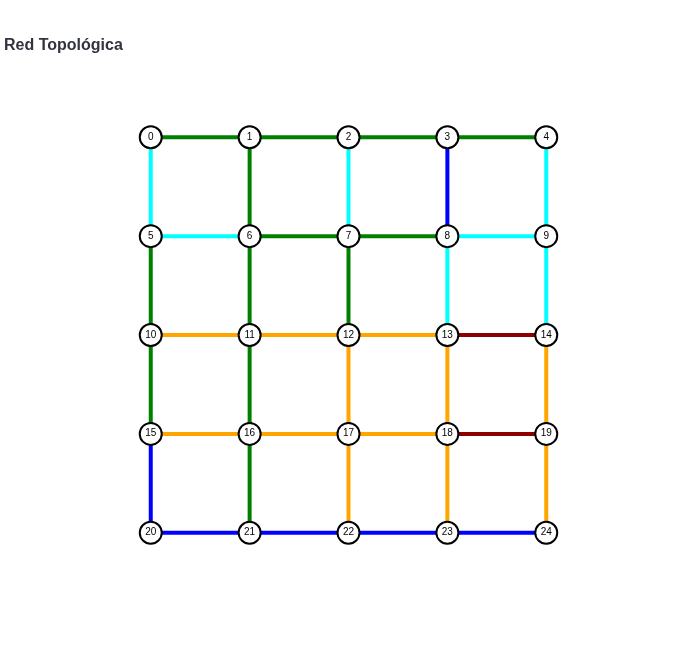
\includegraphics[width=\columnwidth]{img/red_base.png}
\caption{Grafo representativo de la red base $5 \times 5$ utilizada como entorno de control con costos asimétricos por tubería.}
\label{fig:redbase}
\end{figure}

Para aislar la varianza inherente a la estocasticidad de ambas metaheurísticas, cada configuración fue sometida a un estudio empírico de $15$ ejecuciones independientes (corridas) por algoritmo y por instancia de red.

\subsection{Calibración de Hiperparámetros (Optimización Bayesiana)}
El comportamiento de los sistemas de inteligencia colectiva es altamente sensible a sus hiperparámetros. Para garantizar una competencia justa y optimizar el rendimiento emergente, se aplicó un proceso de calibración mediante Optimización Bayesiana utilizando el framework Optuna. Específicamente, se empleó el muestreador TPE (Tree-structured Parzen Estimator), el cual modela probabilísticamente las regiones del espacio de búsqueda continuo y discreto que arrojan los mejores valores de $Z$.

Tras el proceso de calibración cruzada sobre múltiples semillas aleatorias, el modelo bayesiano determinó un perfil donde el ACO requiere un equilibrio casi simétrico entre el peso del rastro estigmérgico y la visibilidad heurística, priorizando ligeramente la información de los sensores. La configuración extraída resultó en: $\alpha = 1.151$, $\beta = 1.499$, una tasa de evaporación baja $\rho = 0.053$ y una fuerte penalización dinámica $\Omega = 1113.17$.

Cabe destacar que la exploración del espacio paramétrico reveló que esta configuración no es estrictamente única; se identificaron diversas combinaciones de hiperparámetros capaces de minimizar la función de ajuste con rendimientos equivalentes. No obstante, los valores mencionados fueron seleccionados formalmente como el perfil operativo de control para someter a la colonia a la experimentación de la Fase 2.

Por su parte, la Búsqueda Tabú alcanzó su punto de máximo rendimiento con un tamaño de vecindad de $41$ nodos evaluados por iteración, una tenencia en la lista tabú de $23$ pasos y una penalización $\Omega = 675.27$.

% Coordenadas Paralelas (Optuna)
\begin{figure}[htbp]
\centering
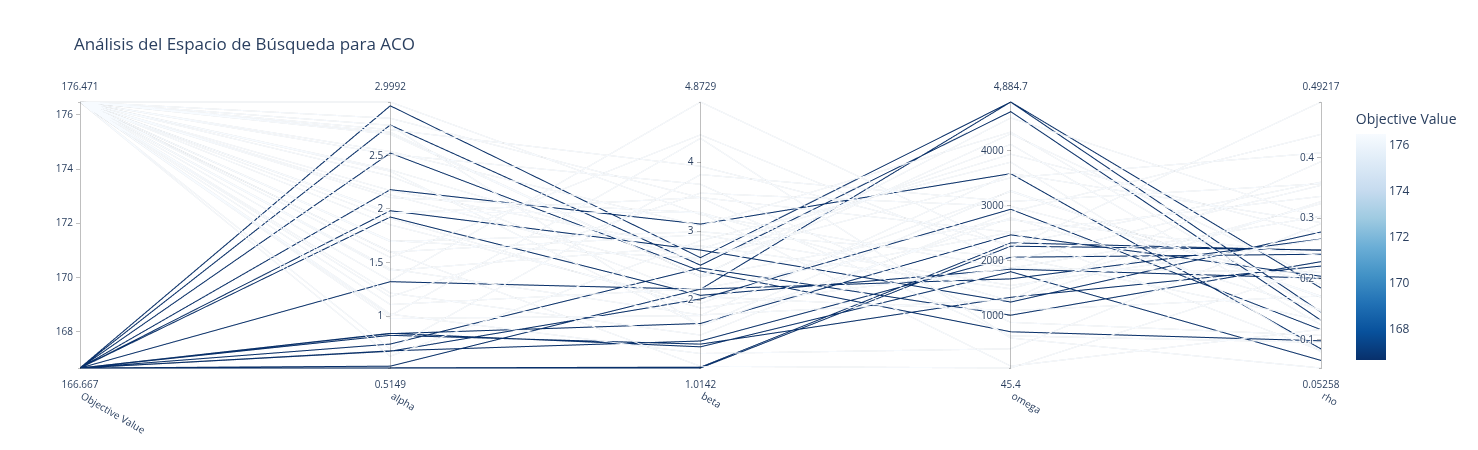
\includegraphics[width=\columnwidth]{img/coordenadas_paralelas.png}
\caption{Exploración del espacio paramétrico, evidenciando la correlación entre las combinaciones de hiperparámetros y la minimización de Z.}
\label{fig:optuna}
\end{figure}

\subsection{Análisis Comparativo de Rendimiento y Robustez}
Los resultados del despliegue en la simulación demostraron una superioridad contundente del enfoque poblacional. Evaluando la calidad global de la exploración, el ACO logró un Fitness Z mediano de $166.67$, superando a la Búsqueda Tabú que obtuvo un puntaje de $176.47$ en su mejor escenario.

Para corroborar la validez estadística de estos hallazgos, se aplicó la prueba no paramétrica de Mann-Whitney U con un nivel de significancia $\alpha = 0.05$. El contraste de medianas entre las 15 ejecuciones independientes arrojó diferencias estadísticamente significativas a favor de ACO en los tres escenarios topológicos evaluados: en la red $5 \times 5$ ($p\text{-valor} = 1.69 \times 10^{-3}$), en la red $10 \times 10$ ($p\text{-valor} = 7.39 \times 10^{-7}$) y, de forma más crítica, en la red asimétrica ($p\text{-valor} = 2.14 \times 10^{-7}$).

La dispersión de las métricas obtenidas no solo confirma que el modelo ACO encuentra soluciones más óptimas de manera global, sino que además presenta una varianza significativamente menor. Esta estrecha agrupación de resultados indica que la inteligencia de enjambre es computacionalmente más robusta y dependiente en menor medida de una semilla estocástica afortunada, logrando eludir los mínimos locales que frecuentemente corrompen las ejecuciones de trayectorias únicas.

% Convergencia
\begin{figure}[htbp]
\centering
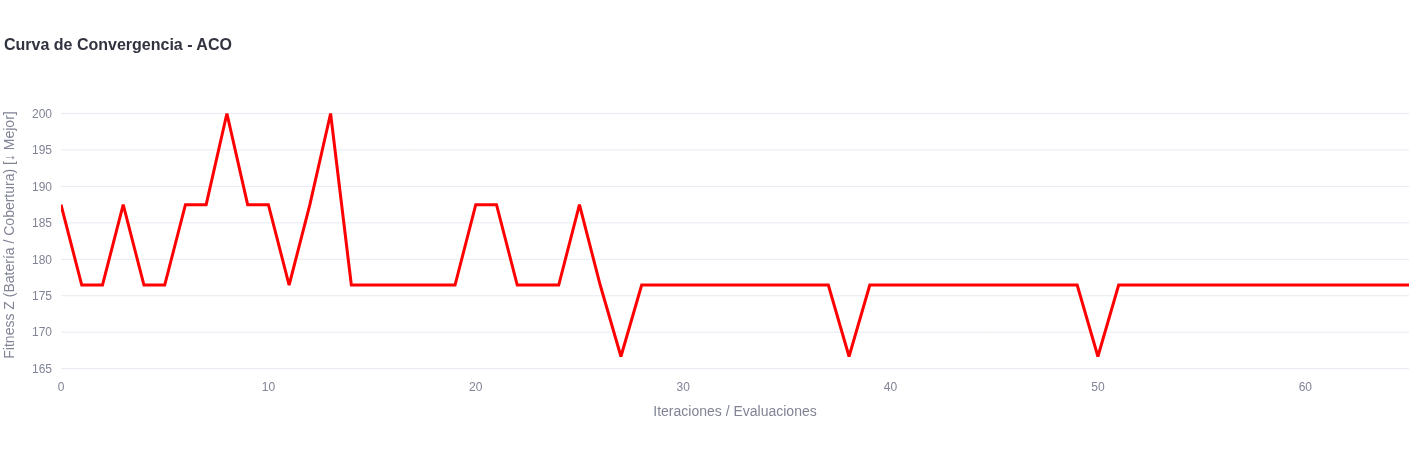
\includegraphics[width=\columnwidth]{img/convergencia_fitness.png}
\caption{Evolución del Fitness a lo largo de las iteraciones, comparando la estabilización del óptimo global en la colonia.}
\label{fig:convergencia}
\end{figure}

% Boxplot / Robustez
\begin{figure}[htbp]
\centering
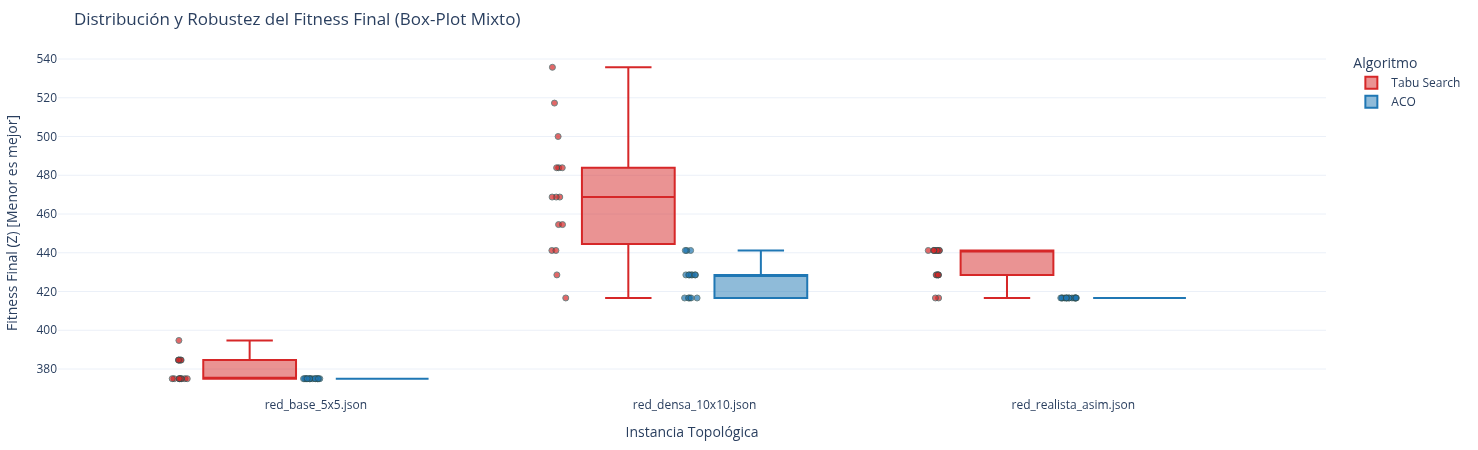
\includegraphics[width=\columnwidth]{img/dispersion_robustez.png}
\caption{Dispersión del Fitness Z en 15 ejecuciones independientes, validando la estabilidad poblacional de ACO frente a TS.}
\label{fig:boxplot}
\end{figure}

\subsection{Eficiencia Energética: El problema del Deadheading}
El análisis pormenorizado del gasto de la batería ($B_{\text{max}}$) revela la principal falencia de las heurísticas clásicas en el problema CARP con penalización de desgaste, dando sustento a la Hipótesis 2.

En topologías complejas (como la red asimétrica o con callejones sin salida), la Búsqueda Tabú sufre el colapso de su memoria a corto plazo. Al llenar su lista de tenencia con los arcos circundantes, el algoritmo se ve acorralado en mínimos locales. Para escapar de estos ciclos, se ve forzado a ejecutar movimientos subóptimos sobre arcos previamente visitados. Este desplazamiento, denominado \textit{deadheading}, no incrementa el denominador de la función objetivo (arcos únicos), pero consume el presupuesto energético de manera inactiva. En las simulaciones de peor caso, el vehículo guiado por TS desperdició hasta $100$ unidades completas de batería exclusivamente en costos de fricción por \textit{deadheading}.

Por el contrario, el ACO utiliza su matriz global de feromonas para anticipar y construir ``derivas armónicas''. Al penalizar dinámicamente la visibilidad ($\Omega$) y reforzar las rutas óptimas a largo plazo, la colonia traza recorridos fluidos que evitan las trampas espaciales. Esto se traduce en una pendiente de cobertura diametralmente superior: por cada unidad de energía invertida, el ACO inspecciona una mayor cantidad de infraestructura nueva, relegando el tránsito inactivo a situaciones estrictamente inevitables.

% Ruta Óptima
\begin{figure}[htbp]
\centering
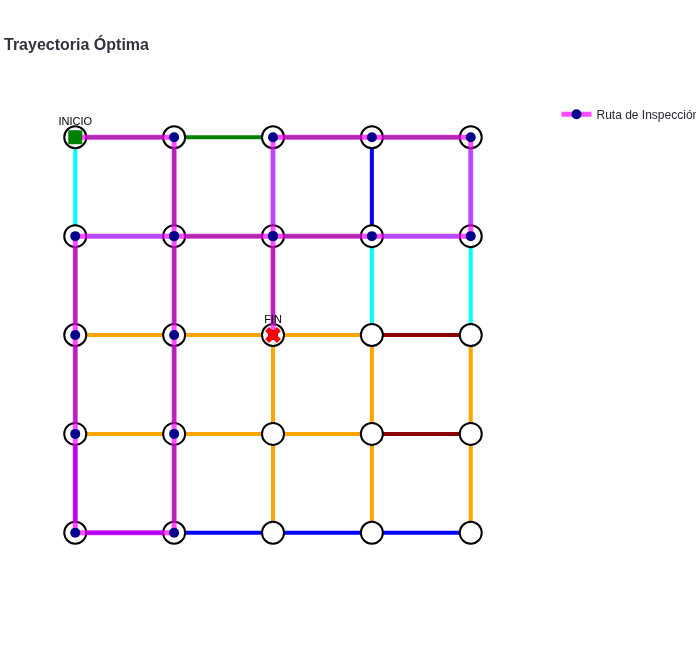
\includegraphics[width=\columnwidth]{img/trayectoria_optima.png}
\caption{Trayectorias propuestas, nótese la evasión de rutas redundantes y rutas de alto costo en la solución generada.}
\label{fig:rutas}
\end{figure}

% Barras (Deadheading)
\begin{figure}[htbp]
\centering
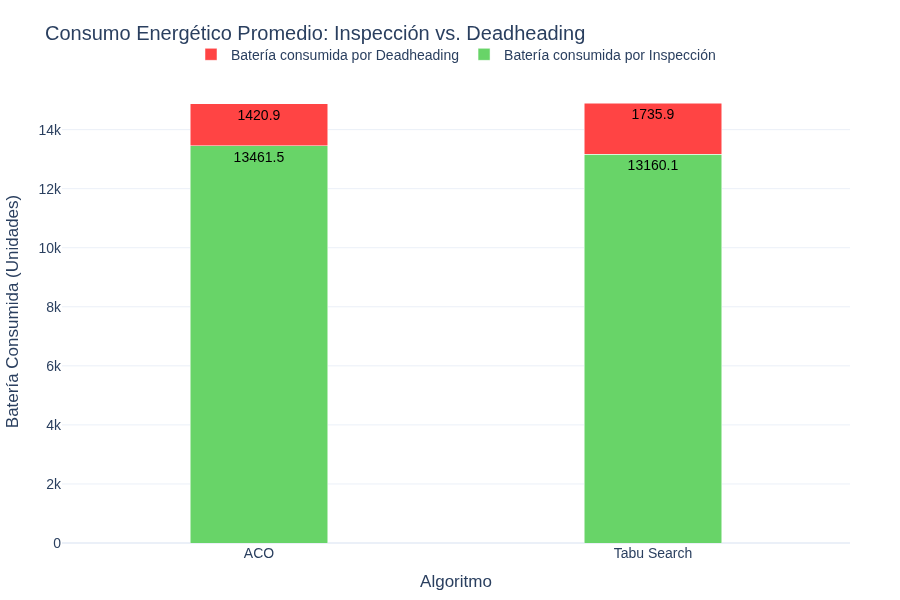
\includegraphics[width=\columnwidth]{img/consumo_energetico.png}
\caption{Desglose de consumo energético total, separando la energía de inspección útil de las pérdidas por fricción inactiva.}
\label{fig:energia}
\end{figure}

\section{Conclusiones y Trabajo Futuro}
El presente trabajo abordó el desafío crítico de planificar trayectorias óptimas para vehículos autónomos de inspección en infraestructuras lineales bajo estrictas restricciones energéticas. La reformulación del Problema de Enrutamiento de Arcos Capacitados (CARP) mediante una función objetivo basada en la capacidad máxima de diseño ($B_{\text{max}}$) permitió penalizar intrínsecamente las detenciones prematuras, garantizando una evaluación algorítmica robusta incluso ante la presencia de callejones sin salida topológicos.

La validación empírica confirmó contundentemente las dos hipótesis rectoras de la investigación. En primer lugar, la fase de calibración mediante optimización bayesiana demostró la viabilidad de perfilar configuraciones de hiperparámetros que equilibran milimétricamente la explotación estigmérgica y la exploración heurística. En segundo lugar, el análisis comparativo evidenció de forma estadísticamente significativa la superioridad de la Optimización por Colonia de Hormigas (ACO) frente a metodologías de trayectoria única, como la Búsqueda Tabú constructiva.

Se concluye que la carencia de un mapeo de feromonas a largo plazo penaliza severamente el rendimiento en redes urbanas asimétricas. Mientras que la memoria a corto plazo de la Búsqueda Tabú colapsa al saturarse su lista de tenencia, derivando en un excesivo desperdicio energético por desplazamientos inactivos (\textit{deadheading}), la inteligencia colectiva del ACO logra estructurar derivas armónicas. La aplicación de la matriz de visibilidad penalizada ($\Omega$) permite a la colonia priorizar la inspección genuina, sorteando los mínimos locales y maximizando la vida útil operativa del dispositivo en campo.

Como líneas de investigación futuras, se proyecta la consolidación de modelos que incorporen disipaciones estocásticas y no lineales de la batería. Asimismo, resulta de especial interés técnico el estudio de sensibilidad paramétrica sobre el propio hardware del vehículo; es decir, evaluar el impacto costo-beneficio de incrementar la capacidad de almacenamiento energético frente a las penalizaciones por el consecuente aumento de masa y fricción en la tubería.

\begin{thebibliography}{00}
\bibitem{b1} G. V. Batista, C. T. Scarpin, J. E. Pécora, y A. Ruiz, ``A New Ant Colony Optimization Algorithm to Solve the Periodic Capacitated Arc Routing Problem with Continuous Moves,'' \textit{Mathematical Problems in Engineering}, vol. 2019, 2019.
\bibitem{b2} T. Akiba, S. Sano, T. Yanase, T. Ohta, y M. Koyama, ``Optuna: A Next-generation Hyperparameter Optimization Framework,'' en \textit{Proceedings of the 25th ACM SIGKDD International Conference on Knowledge Discovery \& Data Mining}, 2019.
\bibitem{b3} B. L. Golden y R. T. Wong, ``Capacitated arc routing problems,'' \textit{Networks}, vol. 11, pp. 305--315, 1981.
\bibitem{b4} E.-G. Talbi, \textit{Metaheuristics: From Design to Implementation}, 1ra ed. Hoboken, NJ, USA: John Wiley \& Sons, 2009.
\end{thebibliography}

\end{document}